\let\negmedspace\undefined
\let\negthickspace\undefined
\documentclass[journal]{IEEEtran}


\setlength{\headheight}{1cm} % Set the height of the header box
\setlength{\headsep}{0mm}     % Set the distance between the header box and the top of the text
 \usepackage[a4paper,margin=10mm, onecolumn]{geometry}
\usepackage{gvv-book}
\usepackage{gvv}
\usepackage{cite}
\usepackage{amsmath,amssymb,amsfonts,amsthm}
\usepackage{algorithmic}
\usepackage{graphicx}
\usepackage{textcomp}
\usepackage{xcolor}
\usepackage{txfonts}
\usepackage{listings}
\usepackage{enumitem}
\usepackage{mathtools}
\usepackage{gensymb}
\usepackage{comment}
\usepackage[breaklinks=true]{hyperref}
\usepackage{tkz-euclide} 
\usepackage{listings}                                       
\def\inputGnumericTable{}                                
\usepackage[latin1]{inputenc}                                
\usepackage{color}                                            
\usepackage{array}                                            
\usepackage{longtable}                                       
\usepackage{calc}                                             
\usepackage{multirow}                                         
\usepackage{hhline}                                           
\usepackage{ifthen}                                           
\usepackage{lscape}
\usepackage{circuitikz}
\tikzstyle{block} = [rectangle, draw, fill=blue!20, 
    text width=4em, text centered, rounded corners, minimum height=3em]
\tikzstyle{sum} = [draw, fill=blue!10, circle, minimum size=1cm, node distance=1.5cm]
\tikzstyle{input} = [coordinate]
\tikzstyle{output} = [coordinate]

\begin{document}

\bibliographystyle{IEEEtran}
\vspace{3cm}

\title{2.6.22}
\author{AI25BTECH11013-Gautham}
 \maketitle
% \newpage
% \bigskip
{\let\newpage\relax\maketitle}

\renewcommand{\thefigure}{\theenumi}
\renewcommand{\thetable}{\theenumi}
\setlength{\intextsep}{10pt} % Space between text and floats


\numberwithin{equation}{enumi}
\numberwithin{figure}{enumi}
\renewcommand{\thetable}{\theenumi}     
\textbf{Question}:\\
Given vectors $\Vec{a} = 2\overrightarrow{i} + \overrightarrow{j} + 3\overrightarrow{k}$ and $\Vec{b} = 3\overrightarrow{i} + 5\overrightarrow{j} - 2\overrightarrow{k}$, find $|\Vec{a} \times \Vec{b}|$.\\

\solution \\

The cross product or vector product of two vectors $\Vec{A} = \myvec{A_{1} \\ A_{2} \\ A_{3}}$ and $\Vec{B} = \myvec{B_{1} \\ B_{2} \\ B_{3}}$ is defined as:
\begin{align}
\Vec{A} \times \Vec{B} = \myvec{
A_{2} B_{3} - A_{3} B_{2}\\
A_{3} B_{1} - A_{1} B_{3} \\
A_{1} B_{2} - A_{2} B_{1}
}
\end{align}

Now, given
\begin{align}
\Vec{a} &= \myvec{2 \\ 1 \\ 3}, \quad
\Vec{b} = \myvec{3 \\ 5 \\ -2}
\end{align}

Using the formula for cross product,
\begin{align}
\Vec{a} \times \Vec{b} &= \myvec{
1 \times (-2) - 3 \times 5 \\
3 \times 3 - 2 \times (-2) \\
2 \times 5 - 1 \times 3
} \\
&= \myvec{
-2 - 15 \\
9 + 4 \\
10 - 3
} \\
&= \myvec{-17 \\ 13 \\ 7}
\end{align}

Finally, the magnitude of the cross product is:
\begin{align}
||\Vec{a} \times \Vec{b}||&= \sqrt{(-17)^2 + 13^2 + 7^2} \\
&= \sqrt{289 + 169 + 49} \\
&= \sqrt{507}
\end{align}

\begin{figure}[h!]
    \centering
    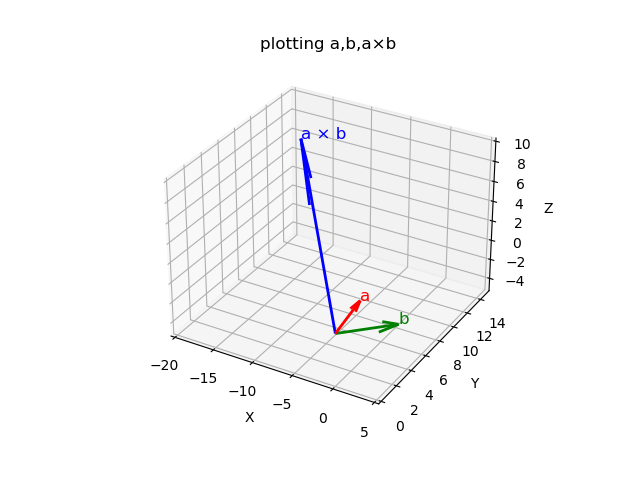
\includegraphics[width=0.8\textwidth]{figs/plot.png}
    \caption{}
    \label{fig:cross product}
\end{figure}

\end{document}
